\chapter{Flash Analysis}
\label{chp:Flash_Analysis}
intro, explain goals
	- consistent flashes, as short as possible
	- consistent capture of flashes
Briefly explain method:
	- Make a device creating and capturing flashes
	- Show flash characteristics
	- Explain how to convert this flash into useful data

\section{Implementation}
\label{sec:Implementation}
A device has been made to generate, receive and analyse flashes. 

\subsection{Flash generator}
The flash generator is a device able to control a LED with high precision. It is able to set

\subsection{Reflection receiver}

\subsection{Analyser}
The analyser will receive the compressed samples from the receiver. The goal of the analyser is to detect patterns in the consecutive flashes and determine

\begin{figure}[!h]
	\includegraphics[width=\textwidth]{pics/systemOverview.png}
	\caption{System overview of the flash generator/analyser}
	\label{fig:systemOveriew}
\end{figure}

\section{Flash characteristics}
\label{sec:Flash_characteristics}

\begin{figure}
	\centering     %%% not \center
	\label{fig:Flashcapturing}
	\subfigure[Test setup in illuminated environment]{\label{fig:a}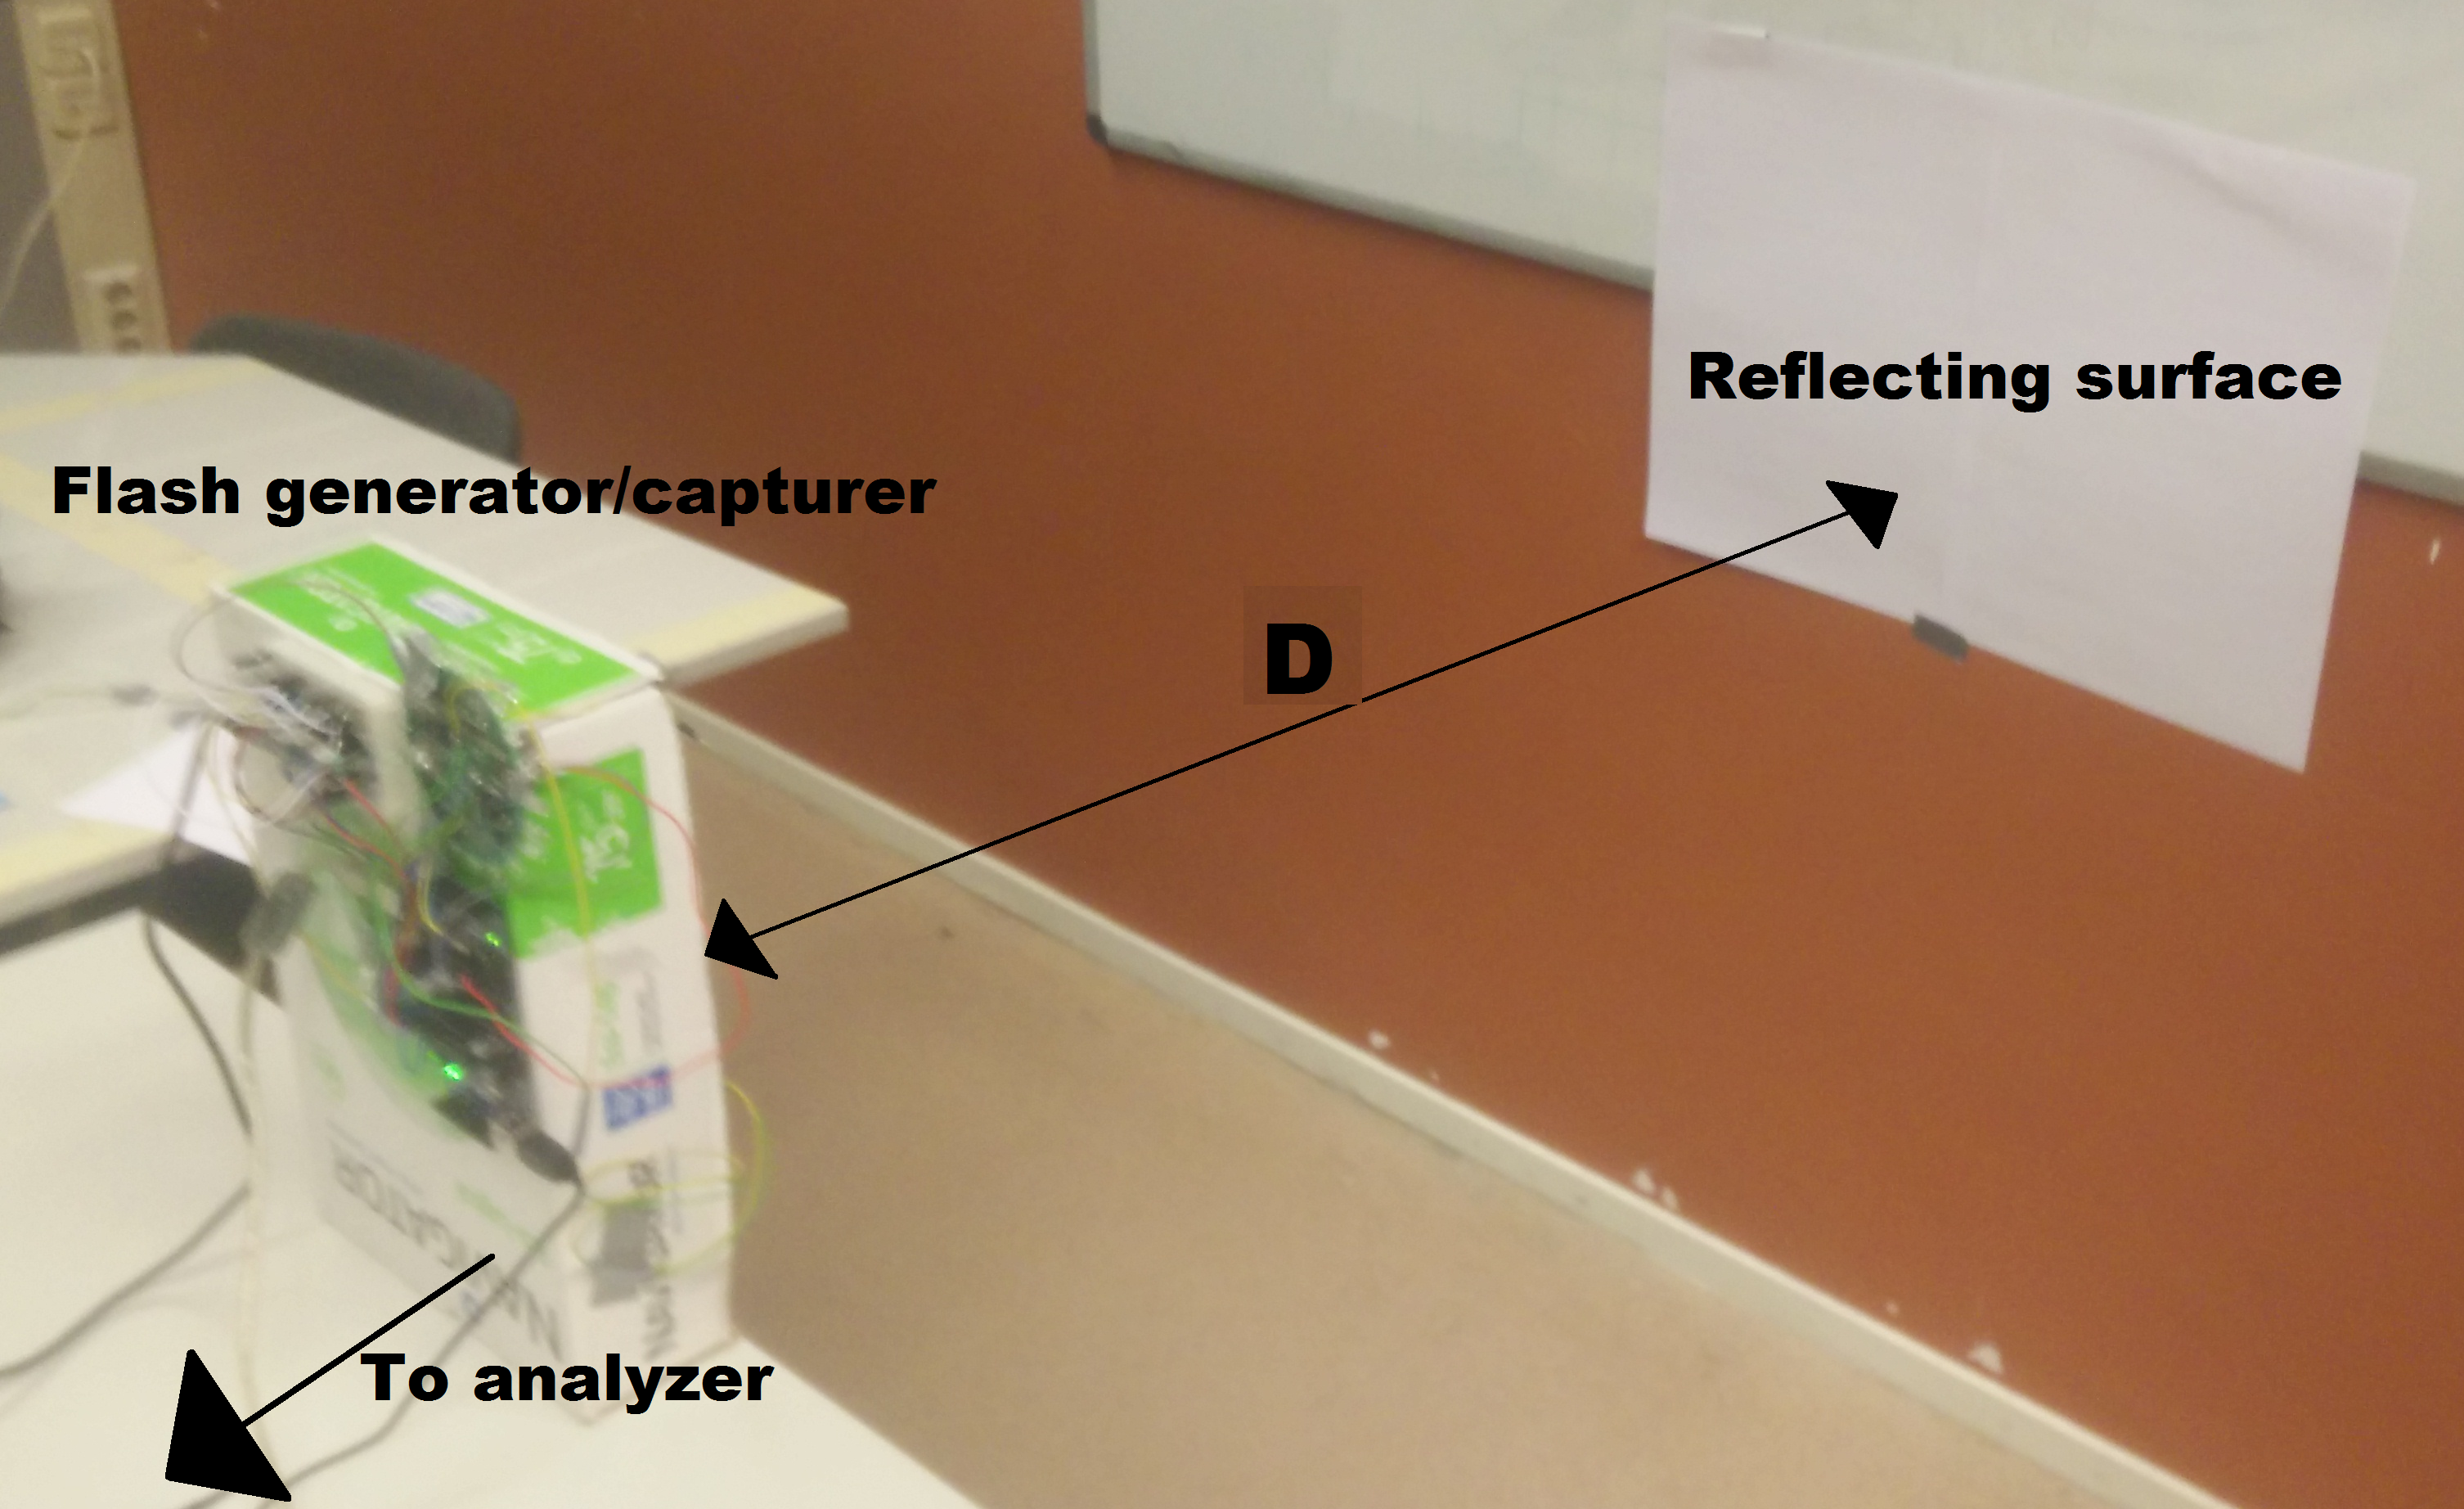
\includegraphics[width=60mm]{pics/Flashcapture_light.png}}
	\subfigure[Test setup in dark environment]{\label{fig:b}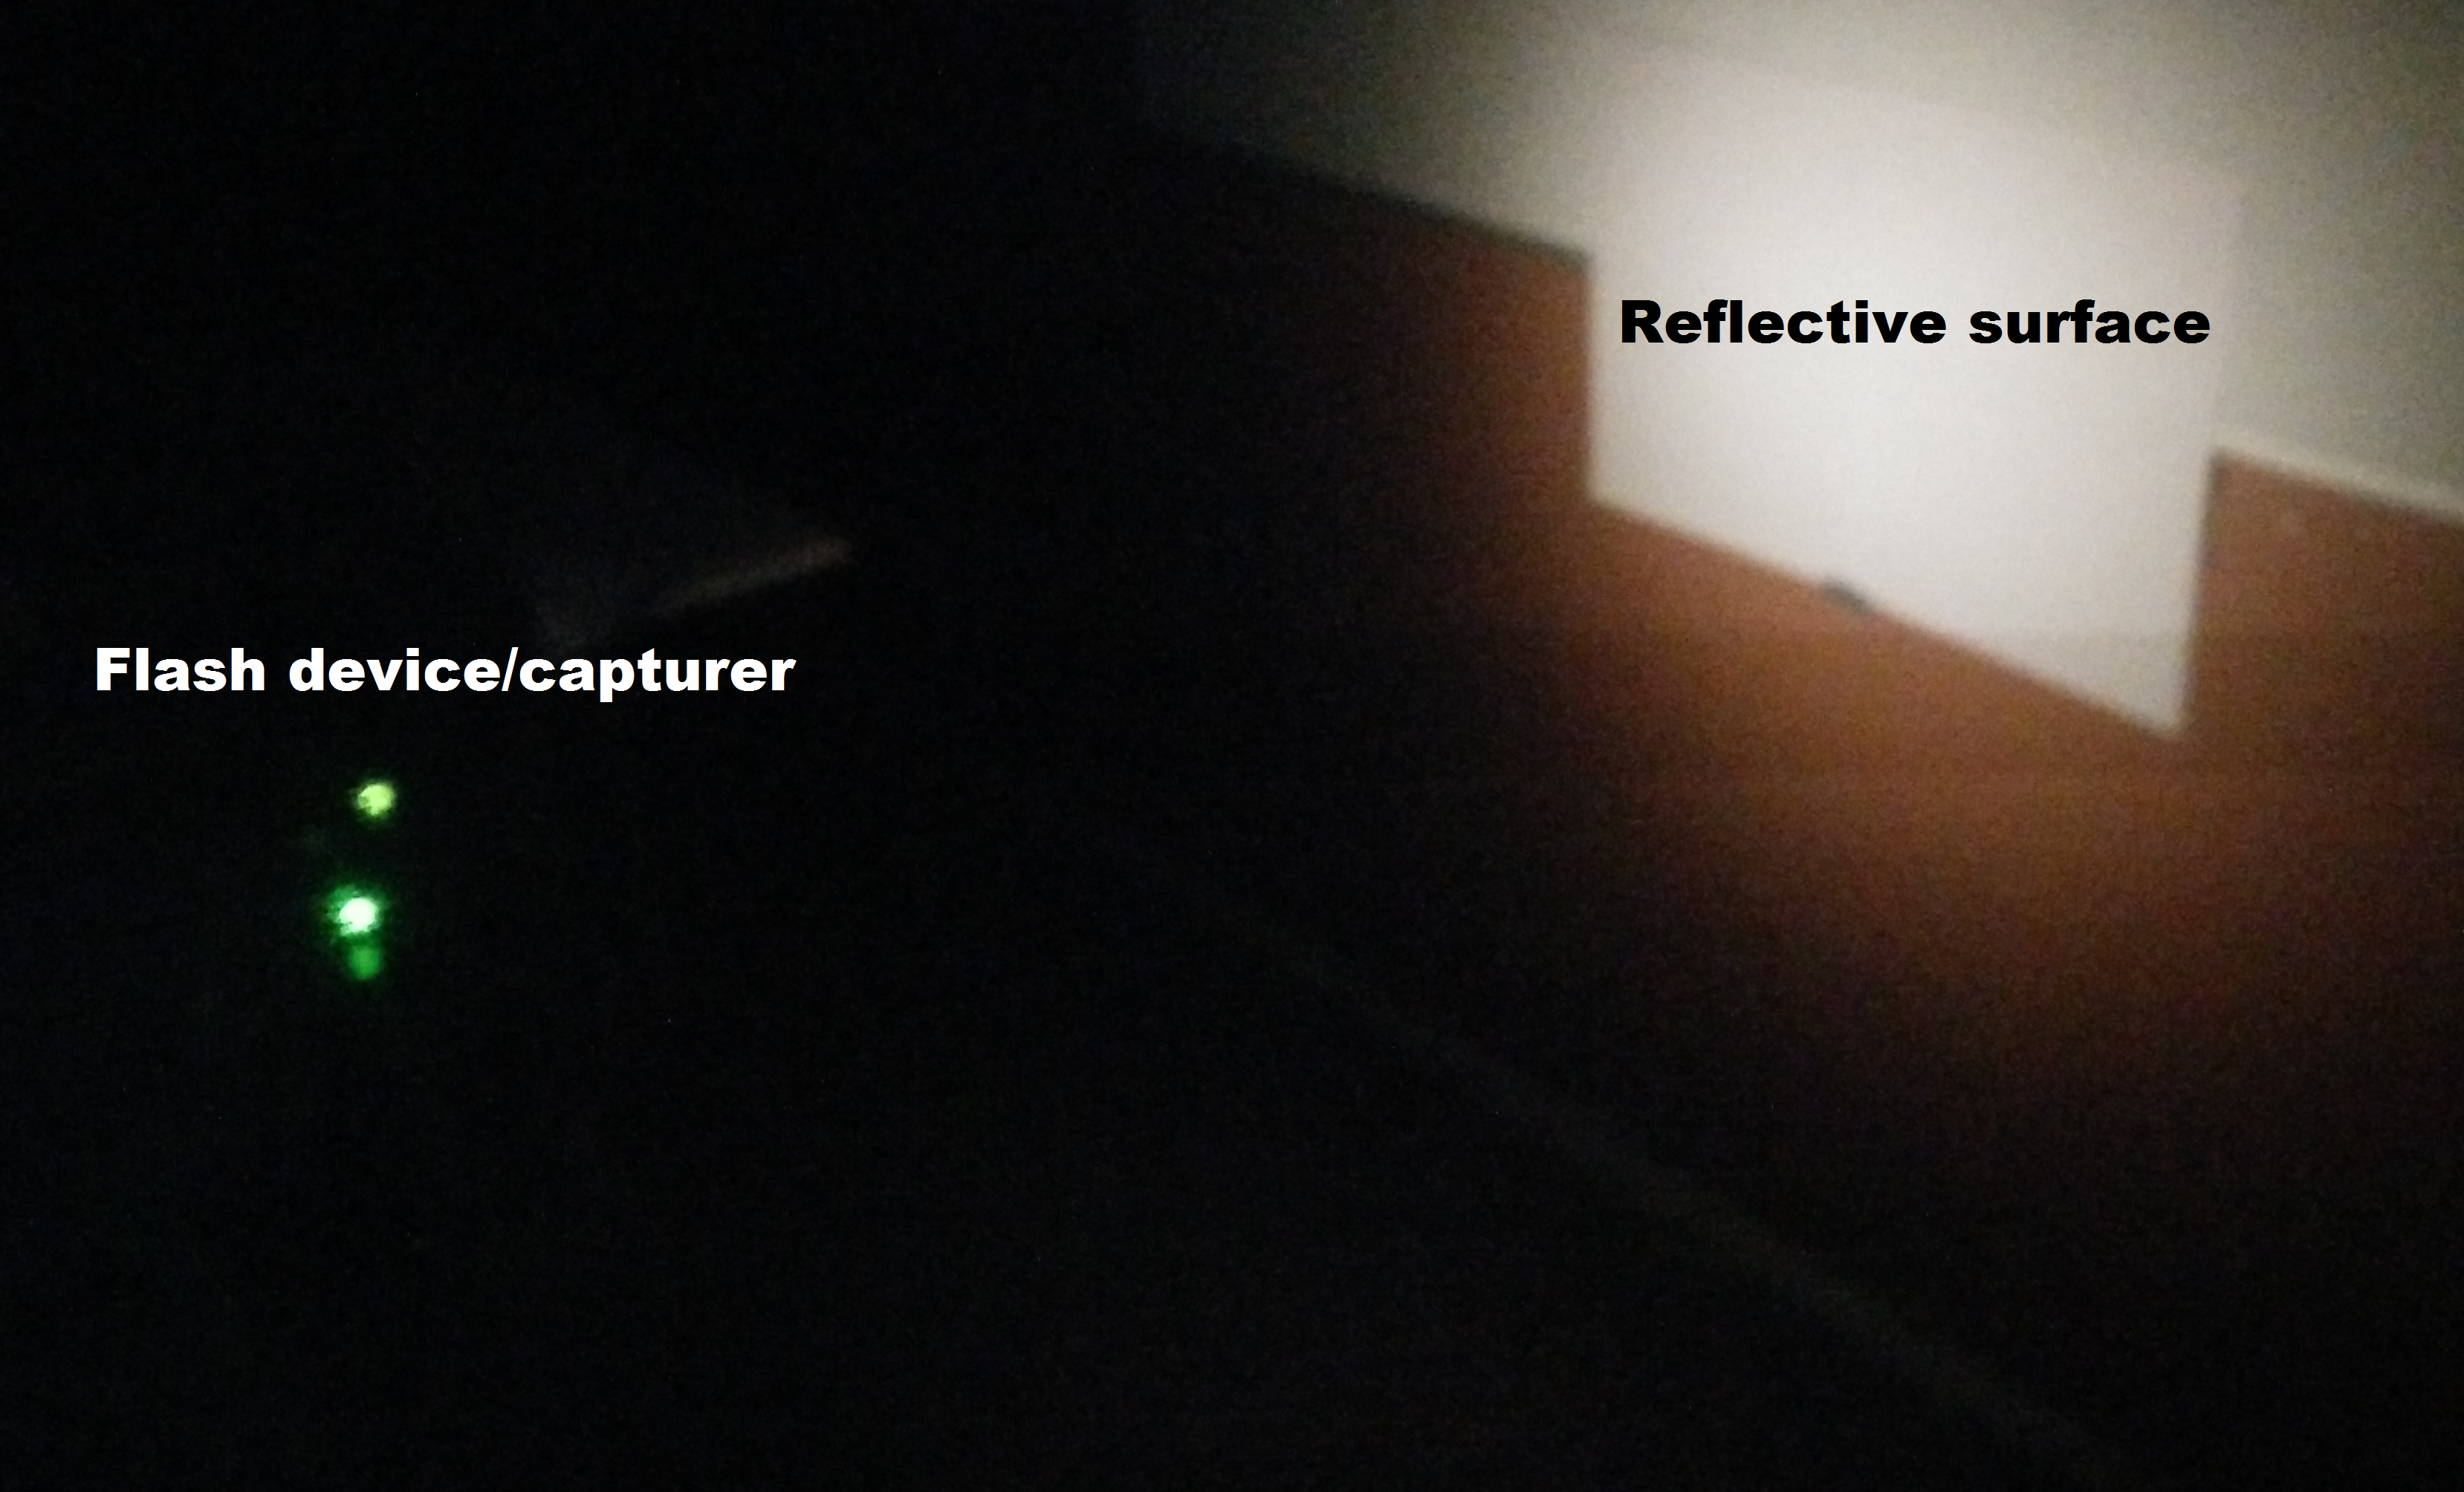
\includegraphics[width=60mm]{pics/Flashcapture_dark.png}}
	\caption{Test setup used to capture flashes in the darkroom.}
\end{figure}

show several captured flashes.
explain extreme ripple.
show real turn on delay time (or in our case, the time we are able to sense the light), rise-time, and turn-off-delay.
Define turn on time.

\begin{figure}[!h]
	\includegraphics[width=\textwidth]{pics/66KhzFilter_placeholder.png}
	\caption{The data captured by the system before and after filtering. @=PLACEHOLDER FIGURE!@.}
	\label{fig:66KhzFilter}
\end{figure}

\subsection{Data generation}
\label{sec:Data_generation}
Show several filtered captured signals in one figure\\
point out the part where light becomes constant\\
pick that t-on time as minimum\\
Mention that a sample of darkness can be taken @ 80 samples.\\
That the number (80) can be reduced by picking a FIR filter instead (less ripple)\\

\subsection{Results and conclusion}
\label{sec:conclusion}
Show the result of several "filtered flashes\\
Explain sources of the "noise", also show FFT and histogram of the noise\\
Explain that the noise could be reduced, but that this would cost a lot more processor time. (which is not recommended to run at 125Hz).\\
Note the noise is approximately Gaussian.

\begin{figure}[!h]
	\includegraphics[width=\textwidth]{pics/histogram_noise_placeholder.png}
	\caption{Histogram of the noise of the data sampled by the system. The distribution roughly follows a normal curve. @=PLACEHOLDER FIGURE!@.}
	\label{fig:histogram_noise}
\end{figure}
